%
% exemplo genérico de uso da classe iiufrgs.cls
% $Id: iiufrgs.tex,v 1.1.1.1 2005/01/18 23:54:42 avila Exp $
%
% This is an example file and is hereby explicitly put in the
% public domain.
%
\documentclass[cic,tc]{iiufrgs}
\usepackage{gensymb}
% Para usar o modelo, deve-se informar o programa e o tipo de documento.
% Programas :
% * cic       -- Graduação em Ciência da Computação
% * ecp       -- Graduação em Ciência da Computação
% * ppgc      -- Programa de Pós Graduação em Computação
% * pgmigro   -- Programa de Pós Graduação em Microeletrônica
%
% Tipos de Documento:
% * tc                -- Trabalhos de Conclusão (apenas cic e ecp)
% * diss ou mestrado  -- Dissertações de Mestrado (ppgc e pgmicro)
% * tese ou doutorado -- Teses de Doutorado (ppgc e pgmicro)
% * ti                -- Trabalho Individual (ppgc e pgmicro)
%
% Outras Opções:
% * english    -- para textos em inglês
% * openright  -- Força início de capítulos em páginas ímpares (padrão da
% biblioteca)
% * oneside    -- Desliga frente-e-verso
% * nominatalocal -- Lê os dados da nominata do arquivo nominatalocal.def


% Use unicode
\usepackage[utf8]{inputenc}   % pacote para acentuação

% Necessário para incluir figuras
\usepackage{graphicx}         % pacote para importar figuras

\usepackage{times}            % pacote para usar fonte Adobe Times
% \usepackage{palatino}
% \usepackage{mathptmx}       % p/ usar fonte Adobe Times nas fórmulas

\usepackage[alf,abnt-emphasize=bf]{abntex2cite}	% pacote para usar citações abnt

%
% Informações gerais
%
\title{Estimativa de profundidade em imagens omnidirecionais}

\author{Dal'Aqua}{Lorenzo Pezzi}

% orientador e co-orientador são opcionais (não diga isso pra eles :))
\advisor[Prof.~Dr.]{Jung}{Claudio}
% \coadvisor[Prof.~Dr.]{Knuth}{Donald Ervin}

% a data deve ser a da defesa; se nao especificada, são gerados
% mes e ano correntes
\date{11 de Janeiro}{2018}

% o local de realização do trabalho pode ser especificado (ex. para TCs)
% com o comando \location:
% \location{Itaquaquecetuba}{SP}

% itens individuais da nominata podem ser redefinidos com os comandos
% abaixo:
% \renewcommand{\nominataReit}{Prof\textsuperscript{a}.~Wrana Maria Panizzi}
% \renewcommand{\nominataReitname}{Reitora}
% \renewcommand{\nominataPRE}{Prof.~Jos{\'e} Carlos Ferraz Hennemann}
% \renewcommand{\nominataPREname}{Pr{\'o}-Reitor de Ensino}
% \renewcommand{\nominataPRAPG}{Prof\textsuperscript{a}.~Joc{\'e}lia Grazia}
% \renewcommand{\nominataPRAPGname}{Pr{\'o}-Reitora Adjunta de P{\'o}s-Gradua{\c{c}}{\~a}o}
% \renewcommand{\nominataDir}{Prof.~Philippe Olivier Alexandre Navaux}
% \renewcommand{\nominataDirname}{Diretor do Instituto de Inform{\'a}tica}
% \renewcommand{\nominataCoord}{Prof.~Carlos Alberto Heuser}
% \renewcommand{\nominataCoordname}{Coordenador do PPGC}
% \renewcommand{\nominataBibchefe}{Beatriz Regina Bastos Haro}
% \renewcommand{\nominataBibchefename}{Bibliotec{\'a}ria-chefe do Instituto de Inform{\'a}tica}
% \renewcommand{\nominataChefeINA}{Prof.~Jos{\'e} Valdeni de Lima}
% \renewcommand{\nominataChefeINAname}{Chefe do \deptINA}
% \renewcommand{\nominataChefeINT}{Prof.~Leila Ribeiro}
% \renewcommand{\nominataChefeINTname}{Chefe do \deptINT}

% A seguir são apresentados comandos específicos para alguns
% tipos de documentos.

% Trabalho Individual [ti]:
% \ti{123}     % numero do TI
% \ti[II]{456} % no caso de ser o segundo TI

%
% palavras-chave
% iniciar todas com letras minúsculas, exceto no caso de abreviaturas
%
\keyword{imagens omnidirecionais}
\keyword{estimativa de profundidade}
\keyword{CNNs}
\keyword{equiretangular}

%\settowidth{\seclen}{1.10~}

%
% inicio do documento
%
\begin{document}

% folha de rosto
% às vezes é necessário redefinir algum comando logo antes de produzir
% a folha de rosto:
% \renewcommand{\coordname}{Coordenadora do Curso}
\maketitle

% dedicatoria
% \clearpage
% \begin{flushright}
%     \mbox{}\vfill
%     {\sffamily\itshape
%       ``If I have seen farther than others,\\
%       it is because I stood on the shoulders of giants.''\\}
%     --- \textsc{Sir~Isaac Newton}
% \end{flushright}

% agradecimentos
%\chapter*{Agradecimentos}
%Agradecimentos...



% resumo na língua do documento
\begin{abstract}
    Abstract em português
\end{abstract}

% resumo na outra língua
% como parametros devem ser passados o titulo e as palavras-chave
% na outra língua, separadas por vírgulas
\begin{englishabstract}{Title in English}{Keywords, in, English}
    Abstract in english
\end{englishabstract}

% lista de figuras
\listoffigures

% lista de tabelas
\listoftables

% lista de abreviaturas e siglas
% o parametro deve ser a abreviatura mais longa
\begin{listofabbrv}{ABREV}
    \item[ABREV] Abreviatura
    \item[SIG] Sigla
\end{listofabbrv}

% idem para a lista de símbolos
\begin{listofsymbols}{$\alpha\beta\pi\omega$}
    \item[$\sum{\frac{a}{b}}$] Somatório do produtório
    \item[$\alpha\beta\pi\omega$] Fator de inconstância do resultado
\end{listofsymbols}

% sumario
\tableofcontents

% aqui comeca o texto propriamente dito

% introducao
\chapter{Introdução}

Este trabalho introduz um método para a estimativa de profundidade a partir de uma única imagem omnidirecional.Imagens omnidirecionais podem ser construídas fazendo uma colagem de várias imagens perspectivas da mesma cena ou capturadas com câmeras específicas para este fim. Também chamadas de imagens esféricas, ou panoramas 360\degree, estas imagens tem ângulo de visão de 360\degree no eixo horizontal e 180\degree no eixo vertical.

A estimativa de profundidade tem múltiplas aplicações em robótica, etc... TODO: aplicações

O método clássico para estimativa de profundidade é o \textit{stereo matching}, onde a informação de disparidade é calculada

% Notas:
% -  Introduzir imagens esféricas, suas utilizações (refs?), profundidade como passo para reconstrução 3D e usos (arquitetura, VR, AR)...

% -



% \section{Exemplos - Figuras e tabelas}

% Esta seção faz referência às Figuras~\ref{fig:estrutura},~\ref{fig:ex1} e~\ref{fig:ex2}, a título de exemplo. A primeira figura apresenta a estrutura de uma figura. A \emph{descrição} deve aparecer \textbf{acima} da figura. Abaixo da figura, deve ser indicado a origem da imagem, mesmo se essa for apenas os autores do texto.

% A Figura~\ref{fig:ex1} representa o caso mais comum, onde a figura propriamente dita é importada de um arquivo ( neste exemplo o formato é \texttt{eps} ou \texttt{pdf}. Veja a seção \ref{sec:fig_format}). A Figura~\ref{fig:ex2} exemplifica o uso do environment \texttt{picture}, para desenhar usando o próprio~\LaTeX.

% \begin{figure}[h]
%     \caption{Descrição da Figura deve ir no topo}
%     \begin{center}
%         % Aqui vai um includegraphics , um picture environment ou qualquer
%         % outro comando necessário para incorporar o formato de imagem
%         % utilizado.
%         \begin{picture}(100,100)
%             \put(0,0){\line(0,1){100}}
%             \put(0,0){\line(1,0){100}}
%             \put(100,100){\line(0,-1){100}}
%             \put(100,100){\line(-1,0){100}}
%             \put(10,50){Uma Imagem}
%         \end{picture}
%     \end{center}
%     \label{fig:estrutura}
%     \legend{Fonte: Os Autores}
% \end{figure}

% \begin{figure}
%     \caption{Exemplo de figura importada de um arquivo e também exemplo de caption muito grande que ocupa mais de uma linha na Lista~de~Figuras}
%     \begin{center}
%         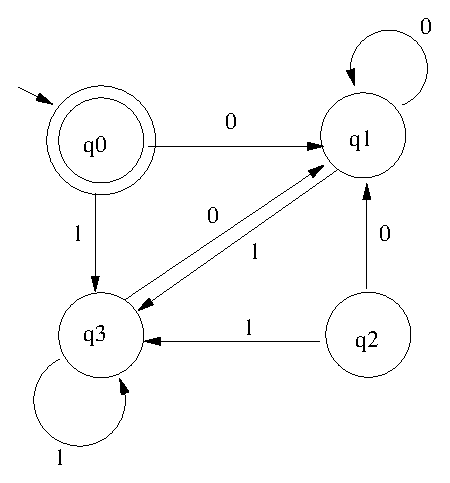
\includegraphics[width=8em]{fig}
%     \end{center}
%     \legend{Fonte: Os Autores}
%     \label{fig:ex1}
% \end{figure}

% % o `[h]' abaixo é um parâmetro opcional que sugere que o LaTeX coloque a
% % figura exatamente neste ponto do texto. Somente preocupe-se com esse tipo
% % de formatação quando o texto estiver completamente pronto (uma frase a mais
% % pode fazer o LaTeX mudar completamente de idéia sobre onde colocar as
% % figuras e tabelas)
% % \begin{figure}[h]
% \begin{figure}
%     \caption{Exemplo de figura desenhada com o environment \texttt{picture}.}
%     \begin{center}
%         \setlength{\unitlength}{.1em}
%         \begin{picture}(100,100)
%             \put(20,20){\circle{20}}
%             \put(20,20){\small\makebox(0,0){a}}
%             \put(80,80){\circle{20}}
%             \put(80,80){\small\makebox(0,0){b}}
%             \put(28,28){\vector(1,1){44}}
%         \end{picture}
%     \end{center}
%     \legend{Fonte: Os Autores}
%     \label{fig:ex2}
% \end{figure}

% Tabelas são construídas com praticamente os mesmos comandos. Ver a tabela \ref{tbl:ex1}.

% \begin{table}[h]
%     \caption{Uma tabela de Exemplo}
%     % OBS: não use \begin{center}, pois este aumenta o espaçamento entre a caption/legend e a tabela
%     % Para figuras, a aparência é melhor com o espaçamento extra
%     \centering
%         \begin{tabular}{c|c|p{5cm}}
%           \hline
%           \textit{Col 1}  &   \textit{Col 2}  &   \textit{Col 3} \\
%           \hline
%           \hline
%           Val 1           &   Val 2           & Esta coluna funciona como um parágrafo, tendo uma margem definida em 5cm. Quebras de linha funcionam como em qualquer parágrafo do tex. \\
%           Valor Longo     & Val 2             & Val 3 \\
%           \hline
%         \end{tabular}
%     \legend{Fonte: Os Autores}
%     \label{tbl:ex1}
% \end{table}

% \subsection{Exemplos - Formato de Figuras}
% \label{sec:fig_format}

% O LaTeX permite utilizar vários formatos de figuras, entre eles \emph{eps}, \emph{pdf}, \emph{jpeg} e \emph{png}. Programas de diagramação como Inkscape (e mesmo LibreOffice) permitem gerar arquivos de imagens vetoriais que podem ser utilizados pelo LaTeX sem dificuldade. Pacotes externos permitem utilizar SVG e outros formatos.

% Dia e xfig são programas utilizados por dinossauros para gerar figuras vetoriais. Se possível, evite-os.

% \subsection{Classificação dos etc.}

% O formato do instituo de informática define 5 níveis: capítulo, seção, subseção e outros 2 sem nome.

% \subsubsection{Subsubseção}
% Exemplo de uma subsubseção.

% \paragraph{Parágrafo}
% Exemplo de um parágrafo.

% \section{Sobre as referências bibliográficas}

% A classe \emph{iiufrgs} faz uso do pacote \emph{abnTeX2} com algumas alterações
% feitas por Sandro Rama Fiorini. Culpe ele se algo der errado. Agradeça a ele
% pelo que der certo. As modificações dão uma camada de tinta NATBIB-style,
% já que o abntex2 usa uns comandos de citação feitos para alienígenas de 5 braços
% wtf. Exemplos de citação:

% \begin{itemize}
%     \item \emph{cite}: Unicórnios são verdes \cite{Adams2009Conceptual};
%     \item \emph{citep}:Unicórnios são verdes \citep{Adams2009Conceptual};
%     \item \emph{citet}: Segundo \citet{Adams2009Conceptual}, unicórnios são
%     verdes.
%     \item \emph{citen or citenum}: Segundo \citen{Adams2009Conceptual},
%     unicórnios são verdes.
%     \item \emph{citeauthor e citeyearpar}: Segundo artigos de
%     \citeauthor{Adams2009Conceptual} , unicórnios são verdes
%     \citeyearpar{Adams2009Conceptual}.

% \end{itemize}

% O estilo abnt fornecido antigamente pelo UTUG não é mais recomendado, pois não
% produz saída de acordo com as exigências da biblioteca.

% Recomenda-se o uso de bibtex para gerenciar as referências (veja o arquivo
% biblio.bib).

% \section{Mais uma Seção}

% Agora vamos fazer várias seções para termos valores de 2 dígitos no \contentsname.

% \section{Mais uma Seção}
% \section{Mais uma Seção}


% e aqui vai a parte principal
%
\chapter{Estado da arte}
\chapter{Nosso método}
\chapter{Resultados}
\chapter{Conclusão}

% referências
% aqui será usado o environment padrao `thebibliography'; porém, sugere-se
% seriamente o uso de BibTeX e do estilo abnt.bst (veja na página do
% UTUG)
%
% observe também o estilo meio estranho de alguns labels; isso é
% devido ao uso do pacote `natbib', que permite fazer citações de
% autores, ano, e diversas combinações desses

\bibliographystyle{abntex2-alf}
\bibliography{biblio}

\end{document}
